\documentclass{beamer}
%\documentclass[aspectratio=169]{beamer}
\usepackage{ctex, hyperref}
\usepackage[T1]{fontenc}
\usepackage{graphicx}
\usepackage{subfigure}

\usepackage{wrapfig}
% other packages
\usepackage{latexsym,amsmath,xcolor,multicol,booktabs,calligra}
\usepackage{graphicx,pstricks,listings,stackengine}

\author{nature communications\hspace{1.5em} \newline25 Sep 2020}
\title{Combining mechanistic and machine learning models for predictive engineering and optimization of tryptophan metabolism}
\institute{Jie Zhang, Søren D Petersen, Tijana Radivojevic, et al. }
\date{Reporter: Jiawei Hwang}
\usepackage{PekingU}





% defs
\def\cmd#1{\texttt{\color{red}\footnotesize $\backslash$#1}}
\def\env#1{\texttt{\color{blue}\footnotesize #1}}
\definecolor{deepblue}{rgb}{0,0,0.5}
\definecolor{deepred}{rgb}{0.6,0,0}
\definecolor{deepgreen}{rgb}{0,0.5,0}
\definecolor{halfgray}{gray}{0.55}

\lstset{
    basicstyle=\ttfamily\small,
    keywordstyle=\bfseries\color{deepblue},
    emphstyle=\ttfamily\color{deepred},    % Custom highlighting style
    stringstyle=\color{deepgreen},
    numbers=left,
    numberstyle=\small\color{halfgray},
    rulesepcolor=\color{red!20!green!20!blue!20},
    frame=shadowbox,
}

%目录文字大小
\setbeamerfont{subsection in toc}%{size=\tiny}
%改变footnote大小 \setbeamerfont{footnote}{size=\tiny}

%改变caption大小 \setbeamerfont{caption}{size=\scriptsize}

%设置caption自动标号 \setbeamertemplate{caption}[numbered]

%设置subfig的label大小 \usepackage{subfig}

%对水平距离的设置常用 em ,而对垂直距离的设置,如行距,常用 ex
%设置正文字体small
\begin{document}\scriptsize


%设置全文行间距
%\usepackage{setspace}
%\setstretch{1.2} 

%设置全文段落间距
%\setlength{\parskip}{0.05em}

\kaishu
\begin{frame}
    \titlepage
\end{frame}

\begin{frame}
    \tableofcontents[sectionstyle=show,subsectionstyle=show/shaded/hide,subsubsectionstyle=show/shaded/hide]
\end{frame}

\section{Introduction}
\begin{frame}{Author Information}
	    \begin{figure}
		\flushleft
		% Requires \usepackage{graphicx}
		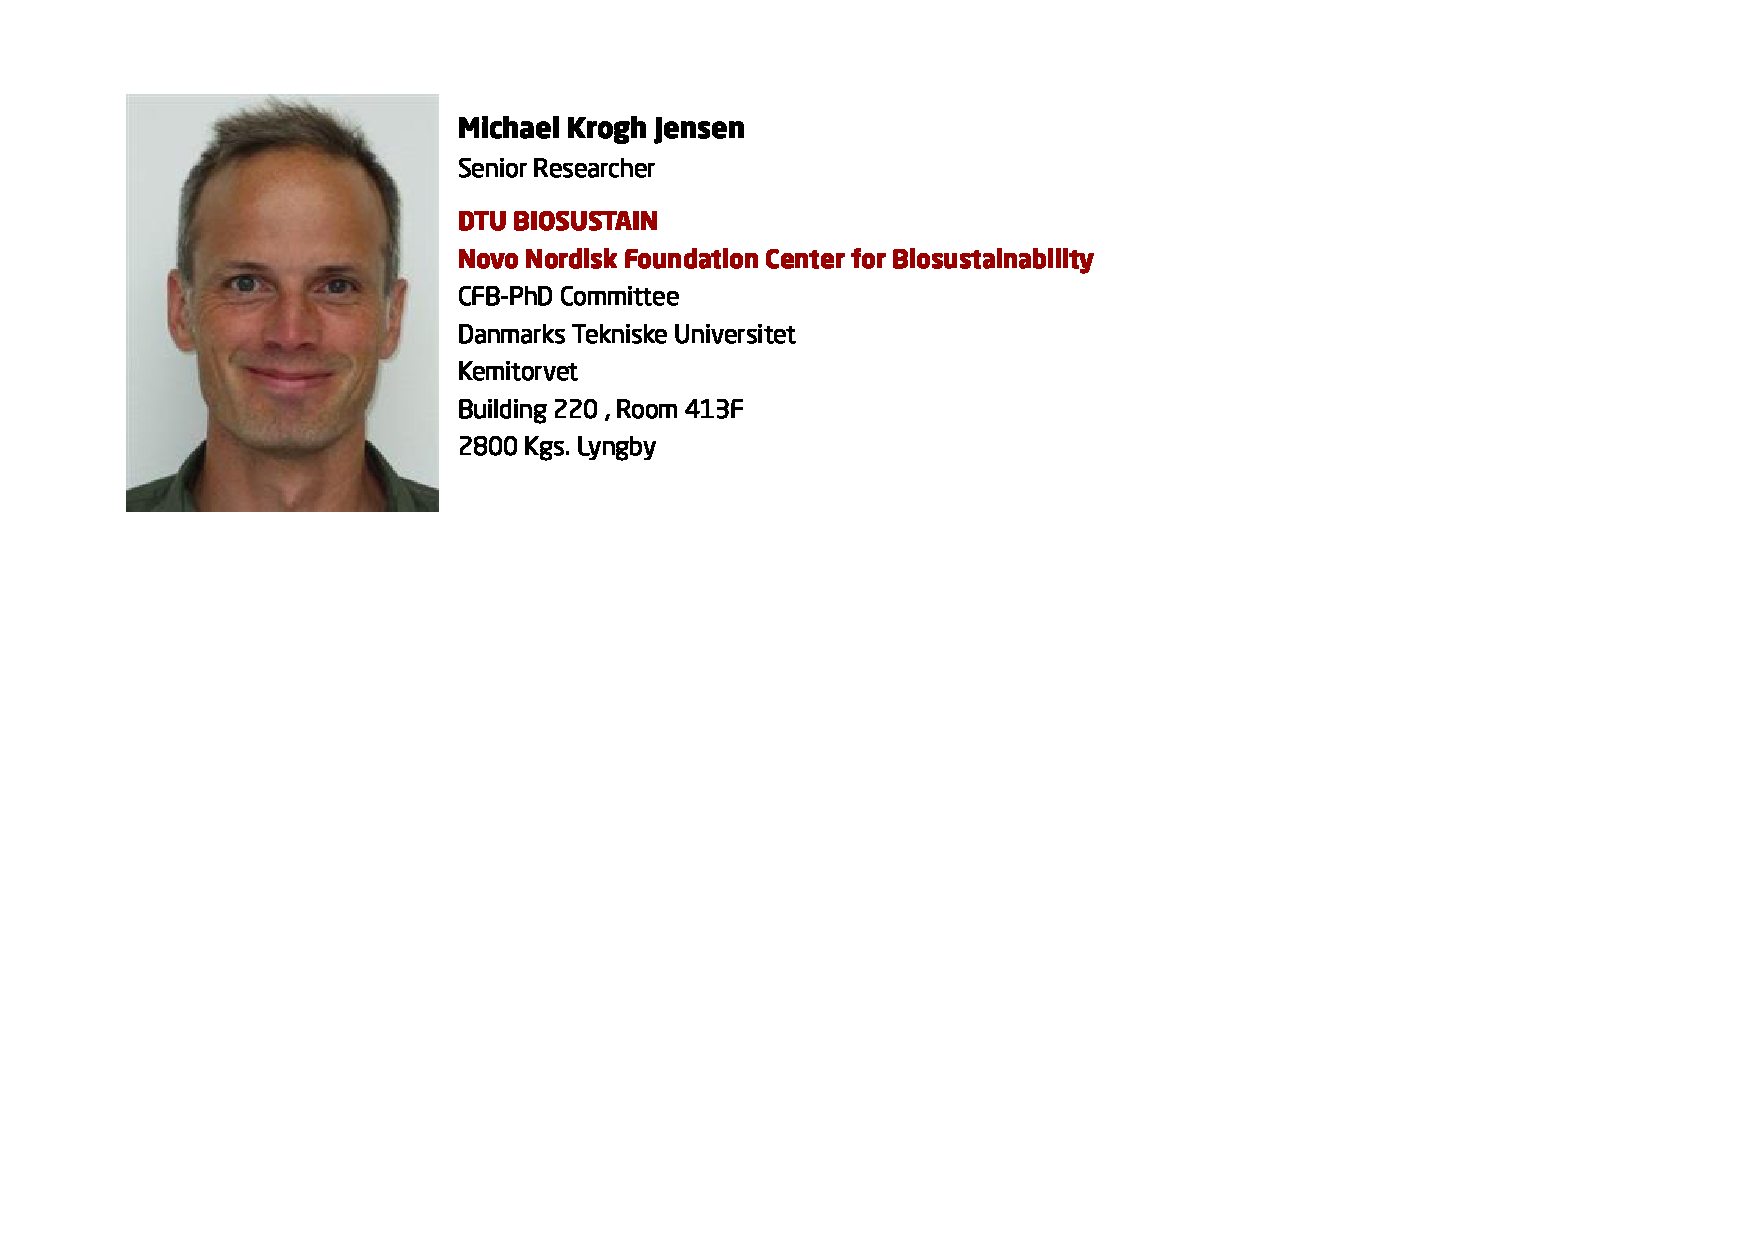
\includegraphics[width=7cm]{pic/Michael Krogh Jensen.pdf}  
 	    \end{figure}
      
    \begin{itemize} [<+-| alert@+>]\zihao {-5} % 当然,除了alert,手动在里面插 \pause 也行
        \item Senior Researcher, Novo Nordisk Foundation Center for Biosustainability
        \item Research Interests: Synthetic Biology Tools for Yeast


    \end{itemize}  
\end{frame}


\begin{frame}{Article Overview}
	    \begin{figure}
		\centering
		% Requires \usepackage{graphicx}
		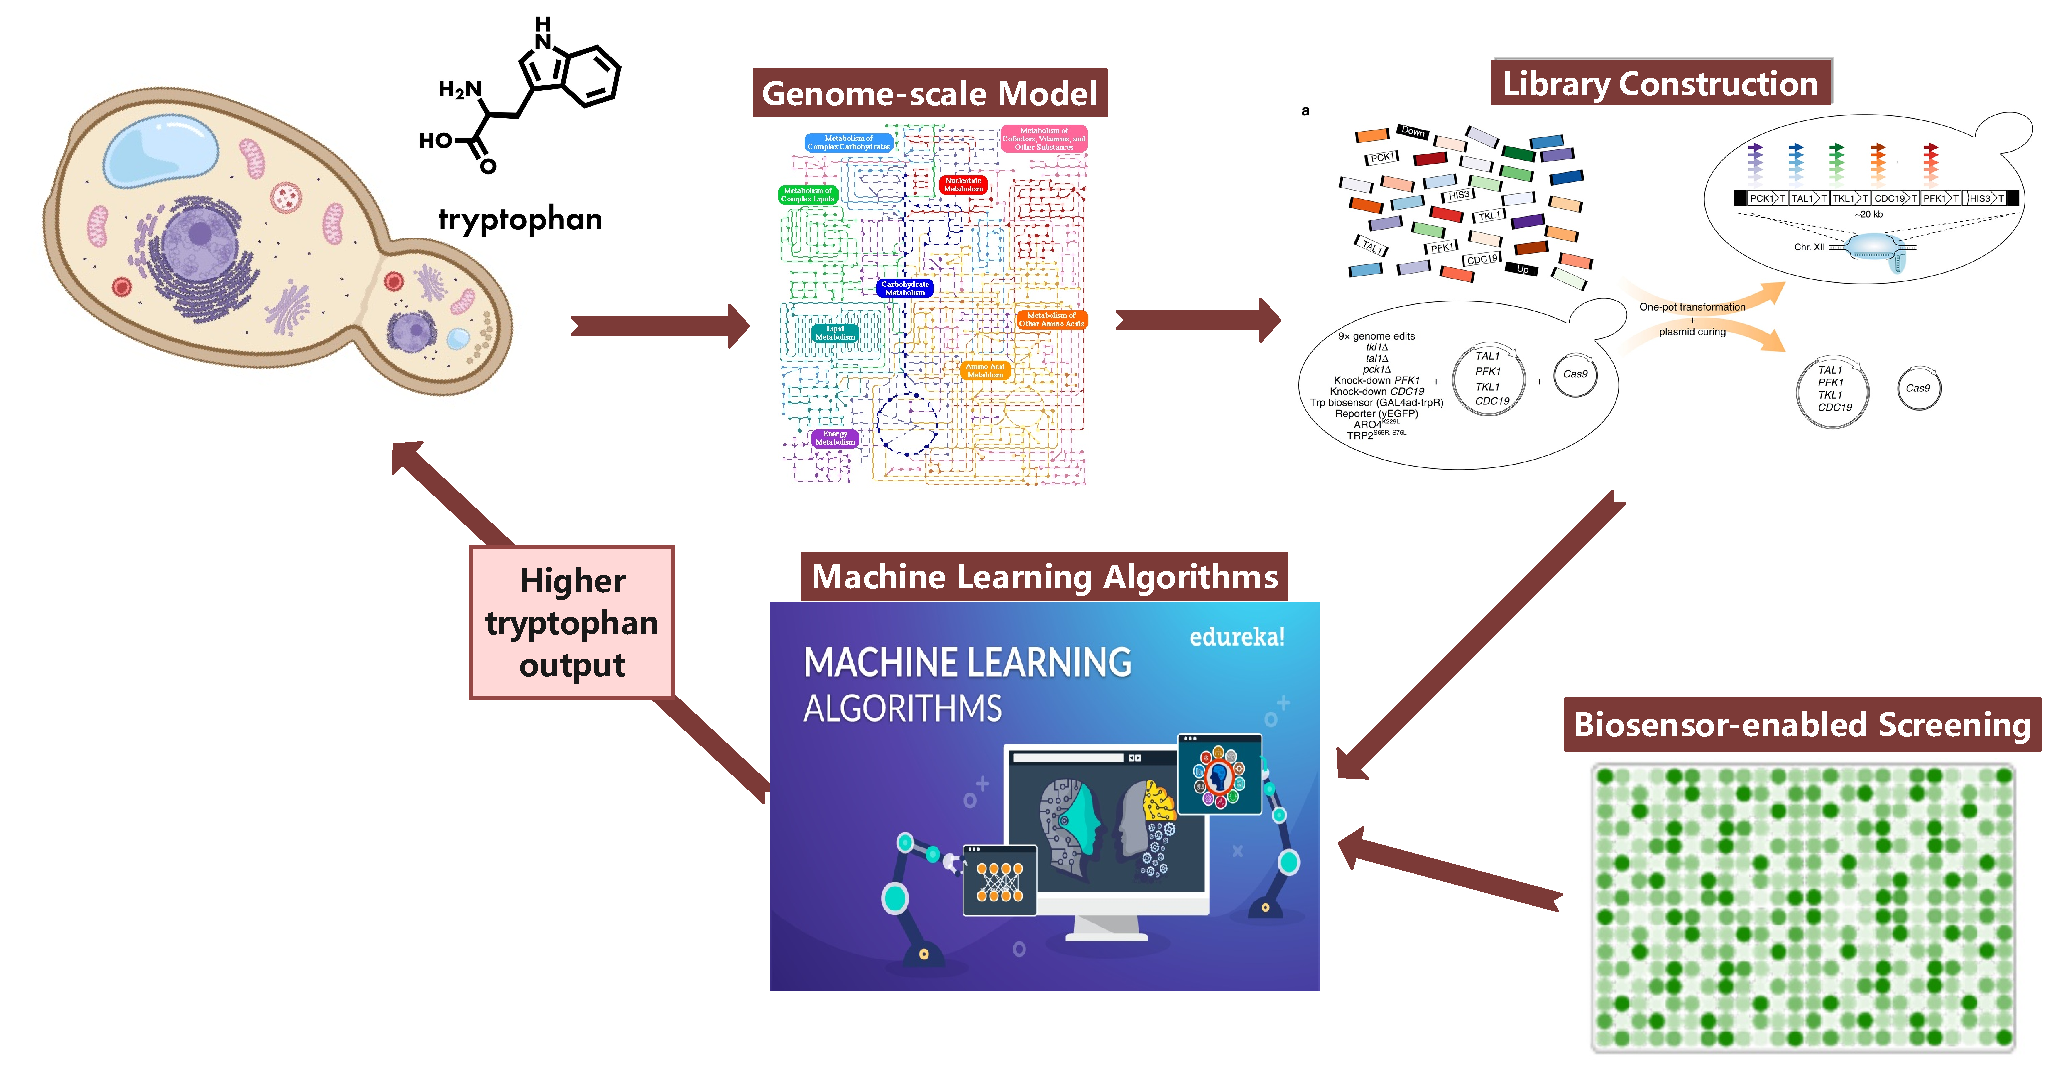
\includegraphics[width=9cm]{pic/abstract.pdf}  
 	    \end{figure}
\end{frame}


\section{Methods}

\begin{frame}{one-pot CRISPR/Cas9-mediated genome editing}
		\begin{columns}
	    \column{0.4\textwidth}
	    \begin{figure}
		\flushleft
		% Requires \usepackage{graphicx}
		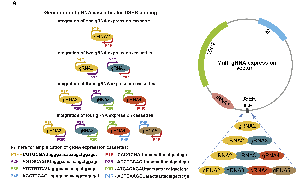
\includegraphics[width=5cm]{pic/onepot.pdf} 
 	    \end{figure}
            \column{0.6\textwidth}      

    \begin{itemize} [<+-| alert@+>]\zihao {-5} % 当然,除了alert,手动在里面插 \pause 也行
        \item  "One-pot CRISPR/Cas9-mediated genome editing" is the use of a single reaction pot, through Cas9-mediated genome editing by CRISPR (Clustered Regularly Interspaced Short Palindromic Repeats), to modify multiple genes simultaneously. This allows for the simultaneous transformation of multiple DNA elements in a single step, making gene editing faster and more efficient.
        \item Efficient, Specific, Versatile

    \end{itemize}    
        \end{columns}


 
\end{frame}



\section{Results}
\subsection{Model-guided design of high tryptophan production.}
\begin{frame}{}
	    \begin{figure}
		\centering
		% Requires \usepackage{graphicx}
		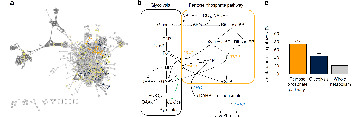
\includegraphics[width=10cm]{pic/图片1.pdf}\\
 	    \end{figure}
    \begin{itemize} [<+-| alert@+>]\zihao {-5} % 当然,除了alert,手动在里面插 \pause 也行
        \item Potential gene targets for tryptophan production were identified using constraint-based modeling, retrieving 192 genes.
        \item The pentose phosphate pathway (PPP) and glycolysis, considered as key pathways, have significantly more gene targets.
        \item Four genes (CDC19, TKL1, TAL1, PCK1) shown to impact shikimate pathway precursors (E4P and PEP) were chosen for combinatorial library construction.
        \item The PFK1 gene, not predicted but selected in the model, can cause carbon flux towards the PPP in various kingdoms due to its insufficient activity.
        
    \end{itemize}  
      
\end{frame}

\begin{frame}{}
	    \begin{figure}
		\centering
		% Requires \usepackage{graphicx}
		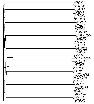
\includegraphics[width=2.5cm]{pic/图片2.pdf}
		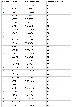
\includegraphics[width=1.8cm]{pic/图片3.pdf}
		
\includegraphics[width=6cm]{pic/图片4.pdf}
 	    \end{figure}
    \begin{itemize} [<+-| alert@+>]\zihao {-5} % 当然,除了alert,手动在里面插 \pause 也行
        \item Promoter selection from transcriptomics datasets focused on well-characterized, sequence-diverse promoters.
        \item  The selection process resulted in 25 sequence-diverse promoters, along with five native promoters, constituting the parts catalog for combinatorial library design.
        
    \end{itemize}  
      
\end{frame}



\subsection{Creation of a platform strain for a combinatorial library.}
\begin{frame}{}
	    \begin{figure}
		\centering
		% Requires \usepackage{graphicx}
		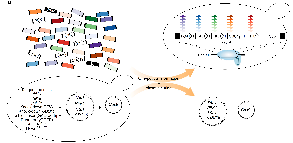
\includegraphics[width=8cm]{pic/图片5.pdf}
 	    \end{figure}  

    \begin{itemize} [<+-| alert@+>]\zihao {-5} % 当然,除了alert,手动在里面插 \pause 也行
        \item\scriptsize Leveraging yeast recombination and CRISPR/Cas9 agility, a sizable combinatorial library was created, equally representing 30 promoters for 5 genes.
        \item\scriptsize  The approach uses sequential deletion of genes and assembly into a genomic landing to overcome low efficiency in targeting multiple loci.
        \item\scriptsize  A galactose-curable plasmid carrying PFK1, CDC19, TKL1 and TAL1 was introduced post-genomic modification, ensuring cell survival and normal growth.
        \item\scriptsize  To enhance AAA accumulation, feedback-resistant enzymes DAHP synthase and anthranilate synthase were integrated into the strain before final assembly of the library.
        
    \end{itemize}  

      
\end{frame}

\subsection{One-pot construction of the combinatorial library.}
\begin{frame}{}
	    \begin{figure}
		\centering
		% Requires \usepackage{graphicx}
		
\includegraphics[width=4.5cm]{pic/图片6.pdf}
		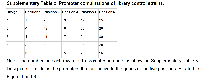
\includegraphics[width=5.5cm]{pic/图片7.pdf}
 	    \end{figure}
    \begin{itemize} [<+-| alert@+>]\zihao {-5} % 当然,除了alert,手动在里面插 \pause 也行
        \item For library construction, the platform strain was transformed with 38 different parts for 7776 unique 20 kb assemblies at the targeted genomic locus.
        \item  To assess assembly fidelity, also transformed yeast with 5 user-defined clusters, including a reference strain with native promoters in front of each of the five selected genes.
        
    \end{itemize}  


\end{frame}


\begin{frame}{}
	    \begin{figure}
		\flushleft
		% Requires \usepackage{graphicx}
		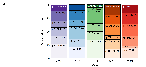
\includegraphics[width=6cm]{pic/图片8.pdf}
		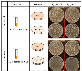
\includegraphics[width=3.5cm]{pic/图片9.pdf}
 	    \end{figure}

    \begin{itemize} [<+-| alert@+>]\zihao {-5} % 当然,除了alert,手动在里面插 \pause 也行
        \item\scriptsize Following transformation, randomly sampled colonies and were successfully cured of the complementation plasmid by using galactose-induced gene expression.
        \item\scriptsize Genotyping identified correctly assembled strains and observed duplicates. 
        \item\scriptsize Based on a Monte Carlo simulation, the expected number of unique genotypes was calculated to be 3759, and all 30 promoters from the one-pot transformation were represented in the genotyped designs.
        \item\scriptsize The results demonstrate high transformation efficiency, high fidelity of parts assembly, and high coverage of the combinatorial library design.
        
    \end{itemize}  
\end{frame}









\subsection{A biosensor for high-throughput library characterization.}
\begin{frame}{}
		\begin{columns}
	    \column{0.16\textwidth}
	    \begin{figure}
		\flushleft
		% Requires \usepackage{graphicx}
		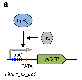
\includegraphics[width=2cm]{pic/图片10.pdf} 
 	    \end{figure}
            \column{0.34\textwidth}
	    \begin{figure}
		\flushleft
		% Requires \usepackage{graphicx}
		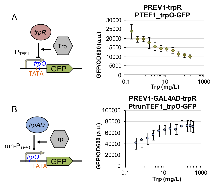
\includegraphics[width=3.6cm]{pic/图片11.pdf}
 	    \end{figure}
            \column{0.5\textwidth}
	    \begin{figure}
		\flushleft
		% Requires \usepackage{graphicx}
		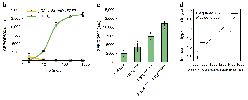
\includegraphics[width=5cm]{pic/图片12.pdf}
 	    \end{figure}
        \end{columns}

%\vspace{-0.6cm}

    \begin{itemize} [<+-| alert@+>]\zihao {-5} % 当然,除了alert,手动在里面插 \pause 也行
        \item\scriptsize Developed a yeast tryptophan biosensor leveraging trpR repressor from Escherichia coli. 
        \item\scriptsize Transformed the trpR repressor into an activator for correlated biosensor-tryptophan readout.
        \item\scriptsize Enhanced strains for high enzyme activities with feedback-resistant versions of ARO4 and TRP2 demonstrated high biosensor outputs.
        \item\scriptsize Validated biosensor as a reliable indicator for tryptophan levels by comparing with HPLC measurements.       
    \end{itemize}  
\end{frame}

\begin{frame}{}
		\begin{columns}
	    \column{0.3\textwidth}
	    \begin{figure}
		\centering
		% Requires \usepackage{graphicx}
		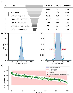
\includegraphics[width=3cm]{pic/图片14.pdf}
  
 	    \end{figure}
            \column{0.7\textwidth}
	    \begin{figure}
		\flushleft
		% Requires \usepackage{graphicx}
            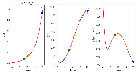
\includegraphics[width=3.6cm]{pic/图片13.pdf}\\
		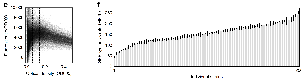
\includegraphics[width=7cm]{pic/图片15.pdf}
 	    \end{figure}
        \end{columns}

    \begin{itemize} [<+-| alert@+>]\zihao {-5} % 当然,除了alert,手动在里面插 \pause 也行
        \item\scriptsize Created biosensor for high-throughput screening of a combinatorial library.
        \item\scriptsize  Observed stable fluorescence per cell at specific OD values and selected this interval for determining GFP synthesis rate.
        \item\scriptsize Discovered that GFP synthesis rate varied sixfold, with an average standard error of the mean of 6.6 MFI/h.
    \end{itemize} 
\end{frame}











\subsection{Using machine learning to predict metabolic pathway designs}


\begin{frame}{}
		\begin{columns}
	    \column{0.4\textwidth}
	    \begin{figure}
		\flushleft
		% Requires \usepackage{graphicx}
		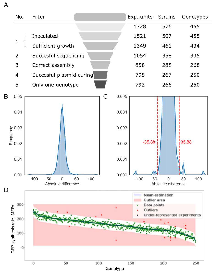
\includegraphics[width=5cm]{pic/图片16.pdf} 
 	    \end{figure}
            \column{0.6\textwidth}
    \begin{itemize} [<+-| alert@+>]\zihao {-5} % 当然,除了alert,手动在里面插 \pause 也行
        \item\scriptsize Combinatorial genetic library and a large phenotypic dataset have been successfully established.
        \item\scriptsize Use of two Machine Learning (ML) algorithms, Automated Recommendation Tool (ART) and EVOLVE algorithm, to predict promoter combinations for improving tryptophan productivity.
        \item\scriptsize Data filtered to maintain quality, resulting in high-quality sequencing and GFP data from 250 genotypes as the input training dataset.
        
    \end{itemize}          
        \end{columns}

\end{frame}



\begin{frame}{}
		\begin{columns}
            \column{0.4\textwidth}
	    \begin{figure}
		\centering
		% Requires \usepackage{graphicx}
		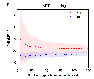
\includegraphics[width=3.3cm]{pic/图片17.pdf}
		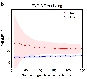
\includegraphics[width=3cm]{pic/图片18.pdf}
 	    \end{figure}
	    \column{0.6\textwidth}
    \begin{itemize} [<+-| alert@+>]\zihao {-5} % 当然,除了alert,手动在里面插 \pause 也行
        \item\scriptsize Both ART and EVOLVE were successful in replicating the data, with an average training mean absolute error (MAE) of 13.8 and 11.9 MFI/h, respectively.
        \item\scriptsize Testing of algorithms' ability to predict production for new promoter combinations through cross-validation; average cross-validated MAE was 21.4 and 22.4 MFI/h for ART and EVOLVE respectively.
        \item\scriptsize ART algorithm found to have slightly smaller uncertainty in MAEs compared to EVOLVE algorithm.
        
    \end{itemize}      
        \end{columns}

\end{frame}

\subsection{Predictive engineering of high tryptophan production.}


\begin{frame}{}
		\begin{columns}
	    \column{0.5\textwidth}
	    \begin{figure}
		\centering
		% Requires \usepackage{graphicx}
		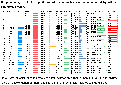
\includegraphics[width=4.8cm]{pic/图片19.pdf} 
 	    \end{figure}
            \column{0.5\textwidth}
	    \begin{figure}
		\centering
		% Requires \usepackage{graphicx}
		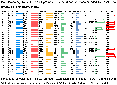
\includegraphics[width=4.8cm]{pic/图片20.pdf}
 	    \end{figure}
        \end{columns}
    \begin{itemize} [<+-| alert@+>]\zihao {-5} % 当然,除了alert,手动在里面插 \pause 也行
        \item\scriptsize Two models (exploitative and explorative) were used to recommend two sets of 30 prioritized designs for high tryptophan production. 
        \item\scriptsize Among the recommendations, two designs overlapped (SP588 and SP627).
        
    \end{itemize} 


\end{frame}


\begin{frame}{}

 
		\begin{columns}
	    \column{0.5\textwidth}
	    \begin{figure}
		\centering
		% Requires \usepackage{graphicx}
		
\includegraphics[width=3cm]{pic/图片21.pdf}\\
		
\includegraphics[width=4cm]{pic/图片22.pdf}
  
 	    \end{figure}
            \column{0.5\textwidth}
	    \begin{figure}
		\centering
		% Requires \usepackage{graphicx}
		
\includegraphics[width=5cm]{pic/图片23.pdf}
 	    \end{figure}
        \end{columns}
    \begin{itemize} [<+-| alert@+>]\zihao {-5} % 当然,除了alert,手动在里面插 \pause 也行
        \item\scriptsize The explorative set of recommendations included eight designs with PGK1 promoter for TKL1 expression control, while the exploitative approach included none. 
        \item\scriptsize Using the same genome engineering approach as for the library construction, 19 individual assemblies of explorative recommendations and 24 exploitative ones were constructed successfully.  
        \item\scriptsize No designs with the PGK1 promoter could be constructed, resulting in a lower number of viable strains found with the explorative approach. 
        
    \end{itemize} 

\end{frame}


\begin{frame}{}
		\begin{columns}
	    \column{0.5\textwidth}
	    \begin{figure}
		\flushleft
		% Requires \usepackage{graphicx}
		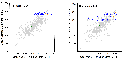
\includegraphics[width=6cm]{pic/图片24.pdf} 
 	    \end{figure}
	    \column{0.5\textwidth}
	    \begin{figure}
		\flushleft
		% Requires \usepackage{graphicx}
		\includegraphics[width=5cm]{pic/图片26.pdf}
 	    \end{figure}
        \end{columns}
    \begin{itemize} [<+-| alert@+>]\zihao {-5} % 当然,除了alert,手动在里面插 \pause 也行
        \item\scriptsize Both the exploitative and explorative models successfully created predictive strain engineering for high-performance GFP synthesis rates. The best recommendation (SP606) showed a 106\% increase compared to the improved platform design (SP507), and 17\% more than the best one (SP271) in the library sample. 
        
    \end{itemize} 
        

\end{frame}

\begin{frame}{}
		\begin{columns}
	    \column{0.5\textwidth}
	    \begin{figure}
		\flushleft
		% Requires \usepackage{graphicx}
		
\includegraphics[width=5.3cm]{pic/图片25.pdf}
 	    \end{figure}
	    \column{0.5\textwidth}
	    \begin{figure}
		\flushleft
		% Requires \usepackage{graphicx}
		
\includegraphics[width=2.6cm]{pic/图片27.pdf}
		
\includegraphics[width=2.6cm]{pic/图片28.pdf}
 	    \end{figure}
        \end{columns}
    \begin{itemize} [<+-| alert@+>]\zihao {-5} % 当然,除了alert,手动在里面插 \pause 也行
        \item\scriptsize The exploitative and explorative approaches varied in their measurement, with the explorative approach including recommendations based on a more diverse set of promoters. 
        \item\scriptsize Both models were successful in predicting tryptophan biosynthesis strain designs, achieving biosynthesis rates beyond those previously observed for training models.    
    \end{itemize} 
\end{frame}




%    \begin{itemize} [<+-| alert@+>]\zihao {-5} % 当然,除了alert,手动在里面插 \pause 也行
%        \item\scriptsize 
%        \item\scriptsize  
%        \item\scriptsize 
%        \item\scriptsize 
%        \item\scriptsize 
%        \item\scriptsize  
%        \item\scriptsize 
%        \item\scriptsize        
%    \end{itemize} 


\section{Discussion}
\begin{frame}{}
	    \begin{figure}
		\flushleft
		% Requires \usepackage{graphicx}
		
\includegraphics[width=4cm]{pic/图片35.pdf}
		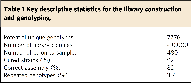
\includegraphics[width=5cm]{pic/图片36.pdf}\\
		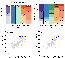
\includegraphics[width=3cm]{pic/图片37.pdf}
		\includegraphics[width=4cm]{pic/图片38.pdf}
		
\includegraphics[width=3cm]{pic/图片40.pdf}
 	    \end{figure}
\end{frame}

\begin{frame}{}

    \begin{itemize} [<+-| alert@+>]\zihao {-5} % 当然,除了alert,手动在里面插 \pause 也行
        \item Combined Approach
            \begin{itemize} [<+-| alert@+>]\zihao {-5} % 当然,除了alert,手动在里面插 \pause 也行
            \item\scriptsize Use of mechanical and machine learning for predictive engineering.
            \item\scriptsize Increased tryptophan production by 74\% and efficiency by 43\%. 
            \end{itemize}
        \item Tool Development 
            \begin{itemize} [<+-| alert@+>]\zihao {-5} % 当然,除了alert,手动在里面插 \pause 也行
            \item\scriptsize Construction of biosensors and strain libraries.
            \item\scriptsize Utilization of one-pot CRISPR/Cas9-mediated genome editing for efficient library construction. 
            \end{itemize}
        \item Machine Learning in Focus
            \begin{itemize} [<+-| alert@+>]\zihao {-5} % 当然,除了alert,手动在里面插 \pause 也行
            \item\scriptsize Application of two machine learning models to predict and guide promoter combinations.
            \item\scriptsize Recognition of the importance of data quality and quantity. 
            \end{itemize}
        \item Potential Improvements
            \begin{itemize} [<+-| alert@+>]\zihao {-5} % 当然,除了alert,手动在里面插 \pause 也行
            \item\scriptsize Enhanced production through fine-tuned fermentation.
            \end{itemize}
        \item Key Findings
            \begin{itemize} [<+-| alert@+>]\zihao {-5} % 当然,除了alert,手动在里面插 \pause 也行
            \item\scriptsize Essential pairing of mechanical and machine learning methods.
            \item\scriptsize Greater prediction power with combined use of genetic selection tools and machine learning. 
            \end{itemize}
        \item Implication
            \begin{itemize} [<+-| alert@+>]\zihao {-5} % 当然,除了alert,手动在里面插 \pause 也行
            \item\scriptsize Achieving efficient design of various cellular systems.
            \end{itemize}
    \end{itemize}

\end{frame}




%\begin{frame}{}
%		\begin{columns}
%            \column{0.1\textwidth}
%	    \column{0.2\textwidth}
%	    \begin{figure}
%		\flushleft
%		% Requires \usepackage{graphicx}
%		
\includegraphics[width=3cm]{pic/图片40.pdf}
 %	    \end{figure}
  %          \column{0.3\textwidth}
%	    \begin{figure}
%		\flushleft
%		% Requires \usepackage{graphicx}
%		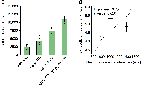
\includegraphics[width=4cm]{pic/图片41.pdf}\\
%		\includegraphics[width=4cm]{pic/图片42.pdf}
% 	    \end{figure}
%            \column{0.4\textwidth}
%	    \begin{figure}
%		\flushleft
%		% Requires \usepackage{graphicx}
%		
\includegraphics[width=3.8cm]{pic/图片43.pdf}\\
%		
\includegraphics[width=3.8cm]{pic/图片44.pdf}\\
%		
\includegraphics[width=3.8cm]{pic/图片45.pdf}
% 	    \end{figure}
%        \end{columns}
%\end{frame}

\begin{frame}
    \begin{center}
        {\Huge\calligra Thanks!}
    \end{center}
\end{frame}

\end{document}
